\documentclass{article}

\title{\Huge Amazon Books Model}
\date{Software Engineering \\  Semester 6 \\  21-03-2020}
\author{Claudiu Rediu 266129\\ \\  Supervisors: Ole Ildsgaard Hougaard\\ \\ VIA University College}
\usepackage{fancyhdr} % Customizable Headers
\usepackage{hyperref}
\usepackage[toc,page]{appendix}
\pagestyle{fancy}
\usepackage{graphicx}
\fancyhf{}
\rhead{
\includegraphics[width=75px]{VIAUniversityLogo.pdf}}
\lhead{Amazon Books Model}
\rfoot{Page \thepage}
\begin{document}
	\pagenumbering{gobble}
	\maketitle
	\newpage
	\pagenumbering{arabic}
	\newpage
	\section*{Model Description}
	The starting point for building our model was the conceptual model of the Amazon Books Database:\newline
	\begin{figure}[h!]
		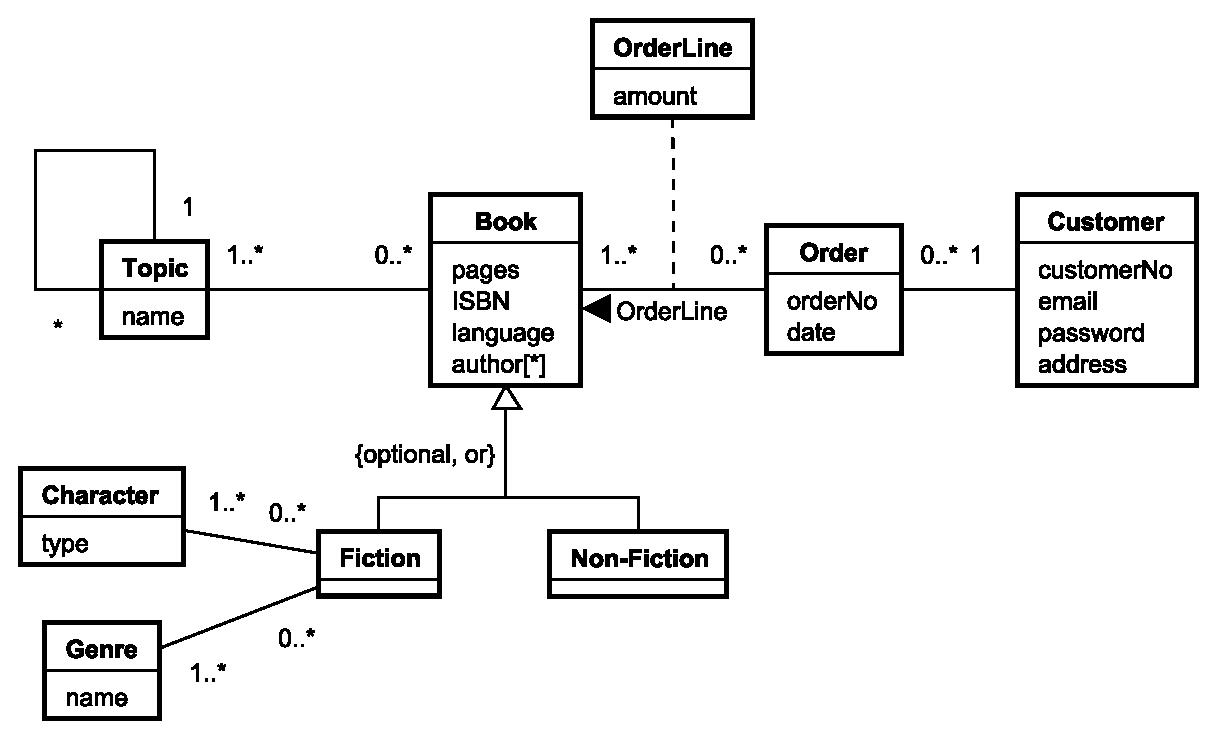
\includegraphics[width=\linewidth]{ConceptualModel.pdf}
		\caption{Conceptual Diagram}
		\label{fig:conceptual}
	\end{figure}
	\newline
	The first choice was in deciding how Topic should handle the recursive relationship. The Parent Reference pattern was chosen because it is the simplest solution and we would like to perform queries to find which has certain parents. \newline
	The second choice was to remove entities, such as OrderLine, because they are no longer needed in many to many relationships. They can be solved by having stored an array of ids in one of the entities depending on the case. All of these relationships were solved in the same way and they didn't require to have the id arrays of each other. \newline
	The third choice was instead of having Fiction and Non-fiction separate, to have a type inside of book, an array of objects for characters and genre separate from book. Genres are not book specific like most characters are. Books are genre specific, so it makes sense that they should be separate. Book will hold the name of the genre that they are part of. The array of objects for characters solution is good as long as there are not a lot of characters included, but usually was is important is the few main characters, so that is why it has been decided to not make it separate from book. \newline
	The fourth choice was having authors just as an array of names. \newline
	The result is the following diagram which describes the relationship between the collections in mongodb:
	\begin{figure}[h!]
		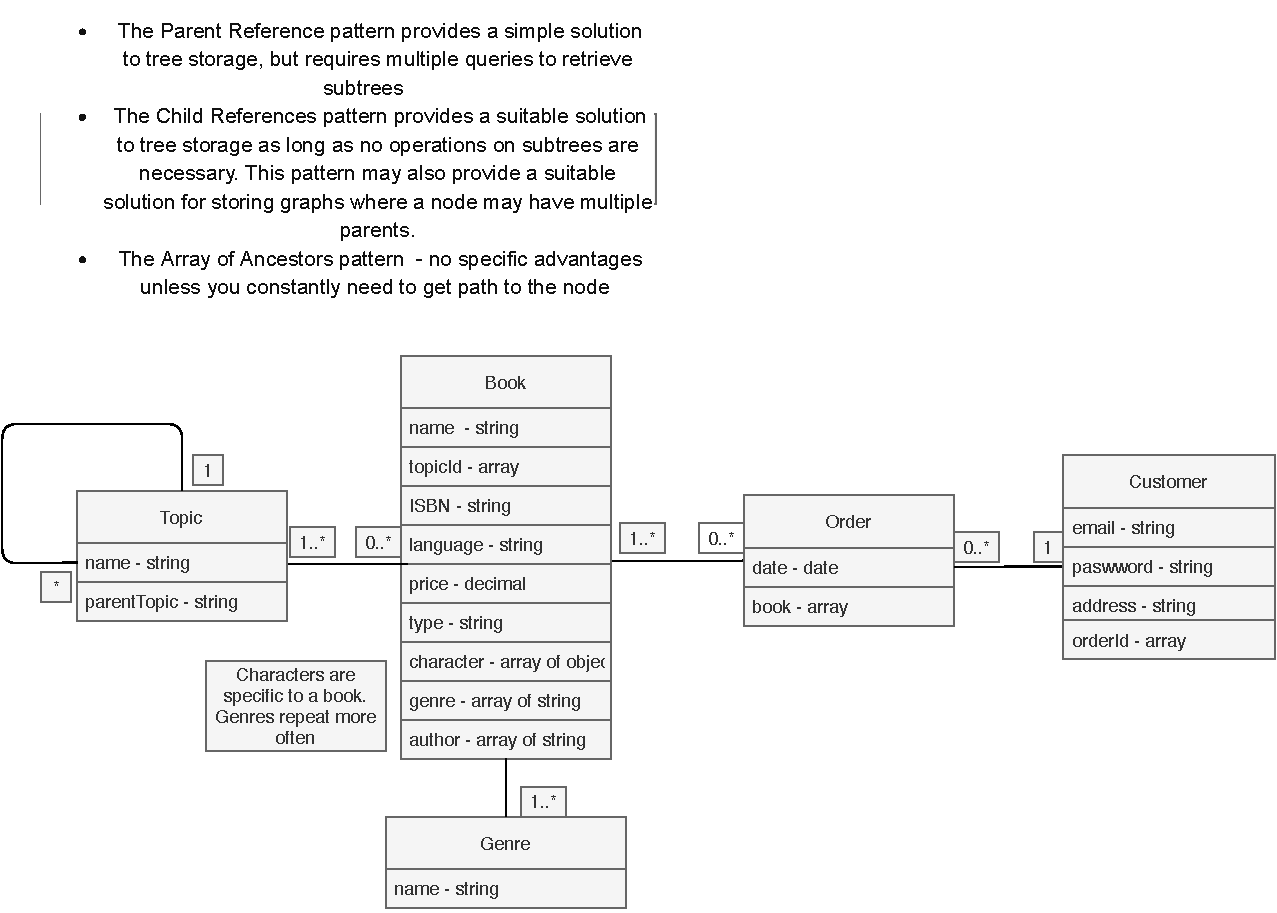
\includegraphics[width=\linewidth]{AmazonMongoDB.pdf}
		\caption{Amazon Books Mongo Diagram}
		\label{fig:Mongo}
	\end{figure}
\end{document}